%--------------------------------------------------------------------sl--------------------
%    PACKAGES AND THEMES
%----------------------------------------------------------------------------------------

\documentclass[aspectratio=169,xcolor=dvipsnames]{beamer}
\usetheme{SimpleDarkBlue}

\usepackage{hyperref}
\usepackage{graphicx} % Allows including images
\usepackage{booktabs} % Allows the use of \toprule, \midrule and \bottomrule in tables

%----------------------------------------------------------------------------------------
%    TITLE PAGE
%----------------------------------------------------------------------------------------

\title{Multi-platform distributed systems
with Aggregate Computing in Kotlin:
the case of proximity messaging}

\author{
    Luca Marchi
    \vspace{0.2cm}
}

\institute
{
    
    \textbf{ALMA MATER STUDIORUM – UNIVERSITÀ DI BOLOGNA} \\
    Corso di Laurea Triennale in Ingegneria e Scienze Informatiche \\
    \vspace{0.3cm}
    \textbf{Relatore}: Prof. Pianini Danilo \\
    \textbf{Correlatore}: Dott.ssa Cortecchia Angela
}


\date{Sessione III Anno Accademico 2024-2025}

%----------------------------------------------------------------------------------------
%    PRESENTATION SLIDES
%----------------------------------------------------------------------------------------

\begin{document}

\begin{frame}
    % Print the title page as the first slide
    \titlepage

\end{frame}

% \begin{frame}{Overview}
%     % Throughout your presentation, if you choose to use \section{} and \subsection{} commands, these will automatically be printed on this slide as an overview of your presentation
%     \tableofcontents
% \end{frame}

%------------------------------------------------

\begin{frame}{Overview and Motivations}
    \begin{columns}[c]

        \column{0.55\textwidth}
        \begin{itemize}
            \item Problem of centralized systems: single point of failure, low resilience, useless in the absence of a network.
            \item Real scenarios: emergencies, crowd messaging, widespread IoT
        \end{itemize}

        \column{0.4\textwidth}
        \begin{figure}
            \fbox{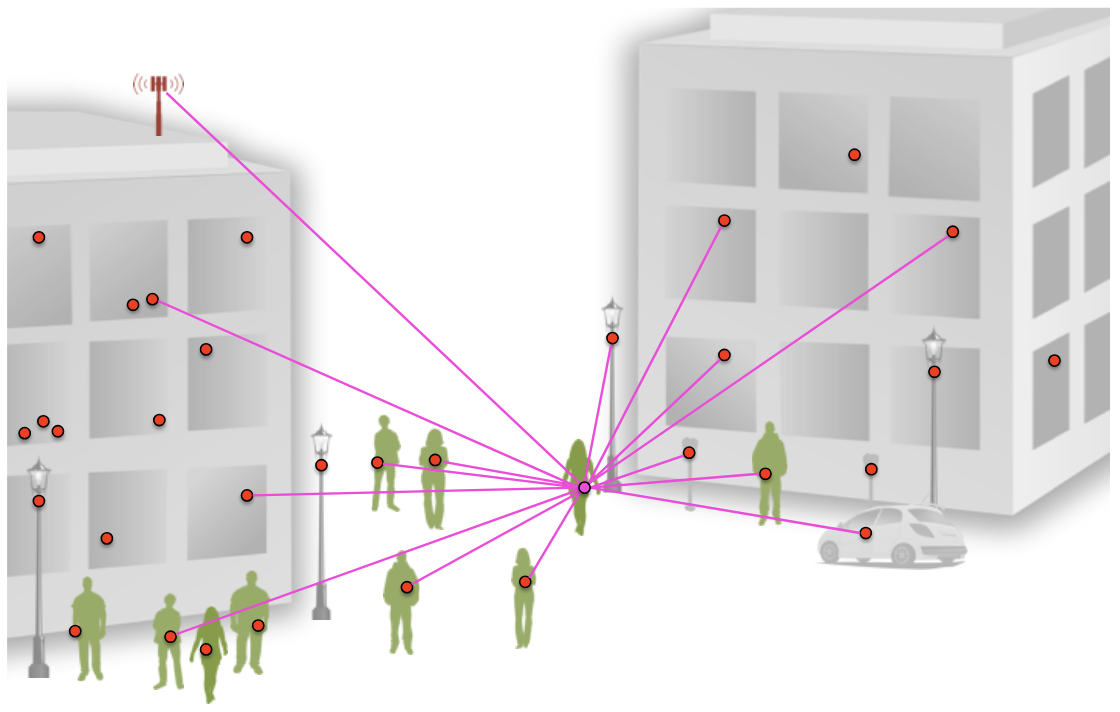
\includegraphics[width=\linewidth]{../thesis/figures/iot-devices.png}}
            \caption{\scriptsize Example of a centralized system for proximity messaging.}
        \end{figure}

    \end{columns}

\end{frame}

%------------------------------------------------

\begin{frame}{Goal}
     \begin{block}{Goal 1}
        Algorithm
    \end{block}

    \begin{block}{Goal 2}
        Multi-platform mobile application with targets Android and iOS.
    \end{block}

\end{frame}

\begin{frame}{Aggregate Computing: The paradigm}
    
    \begin{alertblock}{Aggregate Computing}
        definition
    \end{alertblock}
    
    % In this slide, some important text will be \alert{highlighted} because it's important. Please, don't abuse it.
    
    % \begin{alertblock}{Alertblock}
    %     Sample text in red box
    % \end{alertblock}

    % \begin{examples}
    %     Sample text in green box. The title of the block is ``Examples".
    % \end{examples}
\end{frame}

%------------------------------------------------

\begin{frame}{Project Specifications}
    \begin{block}{Multi-platform support}
        The project must be deployable on multiple platforms and targets.
        
    \end{block}
    \begin{itemize}
        \item \textbf{Aggregate Computing framework}: Collektive
        \item \textbf{Programming language}: Kotlin
        \item \textbf{Multi-platform framework}: Kotlin Multiplatform
        \item \textbf{Simulator}: Alchemist Simulator
    \end{itemize}
    
\end{frame}

%------------------------------------------------

\begin{frame}{Algorithm (Gossip-Gradient)}

\end{frame}

%------------------------------------------------

\begin{frame}{Validation \& CI}

\end{frame}

%------------------------------------------------

\begin{frame}{Mobile Application (Echo)}

\end{frame}

% \begin{frame}[fragile] % Need to use the fragile option when verbatim is used in the slide
%     \frametitle{Citation}
%     An example of the \verb|\cite| command to cite within the presentation:\\~

%     This statement requires citation \cite{p1}.
% \end{frame}
%------------------------------------------------
\begin{frame}{Conclusions \& Future Development}
    
\end{frame}

\begin{frame}
    \Huge{\centerline{\textbf{The End}}}
\end{frame}

%----------------------------------------------------------------------------------------

\end{document}